%\documentclass[11pt, a4paper]{article}
\documentclass[includeheaders]{scrartcl}
\usepackage{scrlayer-scrpage}
\usepackage{hyperref}
\usepackage[utf8]{inputenc}
% Deutsche Silbentrennung
\usepackage[ngermanb]{babel}
% Unterstützung für Farben
\usepackage[dvipsnames]{xcolor}
% Erweiterte Mathematik-Symbole
\usepackage{amsmath,amscd,amssymb}
% Nummerierte Listen
\usepackage{enumerate}
% Erweiterte Bildeinbettungsoptionen
\usepackage{graphicx}
% Typografisch hochwertige Tabellen
%\usepackage{tabularx,ragged2e,booktabs}
\usepackage{tabularx}
% Unterstützung für Unter-Abbildungen (z.B. 2x2-Matrix)
\usepackage{float}
\usepackage{caption}
\usepackage{subcaption}
% Seitenränder
\usepackage{geometry}
\geometry{a4paper,
	left=2.5cm,
	right=2.5cm,
	top=2.5cm,
	bottom=2.5cm}

% Unterstützung für °-Zeichen
\usepackage{textcomp}
\usepackage{gensymb}
% Formatierung von \paragraph und \subparagraph anpassen
\makeatletter
\renewcommand\paragraph{\@startsection{paragraph}{4}{\z@}%
	{-3.25ex\@plus -1ex \@minus -.2ex}%
	{1.5ex \@plus .2ex}%
	{\raggedsection\normalfont\sectfont\size@paragraph}%
}
\renewcommand\subparagraph{\@startsection{subparagraph}{5}{\z@}%
	{-3.25ex\@plus -1ex \@minus -.2ex}%
	{1.5ex \@plus .2ex}%
	{\raggedsection\normalfont\sectfont\size@subparagraph\mdseries}%
}
\makeatother
\usepackage{lastpage}
\setkomafont{pageheadfoot}{\sffamily} 
\sloppy
\parindent0mm
\parskip3mm

\begin{document}
	
	% o - outer, i - inner, c - center -> location of header/footer-element
%\ohead{\includegraphics[scale=0.5]{img/HPI-Logo.png}}
%\ifoot{\includegraphics[scale=0.5]{img/HPI-Logo.png} }
\ifoot{\includegraphics[scale=0.07]{img/logo}}
\cfoot{Modellierung II, \\ Holger Giese, Sommersemester 2016}
\ofoot{\thepage}


	
	\newpage
	
	\title{Entwurfsdokument\\ \small{(Veranstaltung Modellierung II, SoSe 2016)}}
	\date{}
	\author{}
	
	\maketitle
	\begin{table}[H]
		\centering
		\begin{tabular}{lp{7.5cm}}
			\textbf{Projekt:} & Roboterbasiertes Personentransportsystem\\
			&\\
			\textbf{Auftraggeber: }& Prof. Holger Giese \newline Hasso-Platter-Institut \newline Prof.-Dr.-Helmert-Str. 2–3 \newline 14482 Potsdam\\
		&\\
		\textbf{Auftragnehmer: }& Modellierung II – Projektgruppe 5 \newline Prof.-Dr.-Helmert-Str. 2–3 \newline 14482 Potsdam \newline Sebastian Bischoff\\ 
		\end{tabular}
	\end{table}
	
	
	
	\newpage
	
	\begin{table}[H]
		\centering
		\begin{tabularx}{\textwidth}{|p{4cm}|X|p{4cm}|}
			\hline
			Verantwortlichkeit & Name, Vorname & Datum \\ \hline
			Ansprechpartner    & Bischoff, Sebastian & 11.07.2016 \\
			Bearbeitender      & Sauder, Jonathan & 11.07.2016 \\ 
			Bearbeitender      & Lüpke, Fabian & 11.07.2016 \\ 
			Bearbeitender      & Hering, Jonas & 11.07.2016 \\
			Bearbeitender      & Braun, Jakob & 11.07.2016  \\
			Bearbeitender      & Cremerius, Jonas & 11.07.2016 \\
			Bearbeitender      & Wischner, Jakob & 11.07.2016 \\
			Bearbeitender      & Schwenkert, Daniel & 11.07.2016 \\
			Bearbeitender      & Jäkel, Dominik & 11.07.2016 \\
			Bearbeitender      & König, Bastian & 11.07.2016 \\ \hline
		\end{tabularx}
	\end{table}
	
	\newpage
	
	\tableofcontents

\newpage
\section{Abstrakte Architektur}
In diesem Dokument soll ein Transportsystem mit autonom agierenden Transportvehikeln entwickelt werden, welche Notfalltransporte f\"{u}r ein Krankenhaus erledigen. Die Vehikel werden zu einem vom Krankenhaus angegebenen Ort geschickt, um dort einen Patienten abzuholen und danach zur Klinik zu fahren. 

Dieser Entwurf basiert auf der in der Analyse erarbeiteten Spezifikation des Systems.

\begin{figure}[H]
\centering
\includegraphics[width=0.6\textwidth]{img/KomponentendiagrammAbstrakt.png}
\caption{\textcolor{blue}{Durch eigenes Komponentendiagramm ersetzen}}
\label{KomponentendiagrammAbstrakt}
\end{figure}

Da eine Komponente mit dem Namen Robot bereits vorhanden ist, nennen wir die Robot-Hauptkomponente RobitUnit. Dieser Name verdeutlicht, dass jeder physische Roboter im System durch diese Hauptkomponente repr\"{a}sentiert wird.

In diesem Kapitel wird die im Rahmen der Analyse ermittelte Einteilung des Systems in Komponenten strukturiert dargestellt. Hierbei soll auch die Interaktion der Komponenten untereinander verdeutlicht werden.

\subsection{Server}

Der Server verwaltet die Tasks f\"{u}r die RobotUnits und beh\"{a}lt einen st\"{a}ndigen \"{U}berblick \"{u}ber die Positionen der RobotUnits. Er ist f\"{u}r die effiziente Allokation der Auftr\"{a}ge f\"{u}r die RobotUnits zust\"{a}ndig.

\subsubsection{ServerSoftware}

Die Komponente ServerSoftware ist die Verwaltungslogik des Servers. Sie greift auf die servierseitigen Subsysteme zu und stellt die zentrale Anlaufstelle f\"{u}r alle RobotUnits dar. 

Bei einer Anfrage ermittelt sie die passende RobotUnit und sendet die Position des Ziels. 

\subsection{RobotUnit}

Die Komponente RobotUnit sublimiert die RobotSoftware und Hardware (Komponente Robot) als eine Oberkomponente. Sie vereint alle Hard- und Softwareinterfaces dieser Komponenten und leitet die ein- und ausgehenden Nachrichten der RobotSoftware an den Server weiter. Sie dient somit als \"{u}bergeordnete Schnittstelle f\"{u}r die Kommunikation. 

\subsubsection{RobotSoftware}

Die RobotSoftware steuert den Robot an und verwertet seine Sensordaten. Dazu geh\"{o}rt unter anderem die Fahrlogik und die Verwaltung der Battery, damit angenommene Tasks auch komplett ausgef\"{u}hrt werden k\"{o}nnen und die RobotUnit rechtzeitig die ChargingStation erreicht. 

\subsubsection{Robot}

Die Komponente Robot steht f\"{u}r alle hardwaretechnischen Spezifikationen des Robots. Dazu geh\"{o}ren die Fahreinheit und die interne Sensorik so wie die Battery.   
\newpage
\section{Interaktion der Komponenten}
Auf Basis der Analyse Use Cases wird in diesem Kapitel die Interaktion der einzelnen Komponenten aus Kapitel 1 betrachtet. 
Dabei liegt der Fokus vor allem der Interaktion zwischen der RobotUnit und dem Server, wie dessen Austausch mit dem Hospital und der Taxiapp. 
Die Abläufe innerhalb der Komponenten werden dann in Kapitel 8 näher spezifiziert. \\


\subsection*{Interaktion bei Ausführung von \emph{Receive Order \& Cancel Order}}

Elementar ist in diesem Fall der UseCase ReceiveOrder(Use Case 1.1), der es Usern ermöglicht Anfragen oder Notrufe aufzusetzen, um ein Taxi oder einen Krankentransporter anzufordern. 
Das System arbeitet mit einer Warteliste; Krankentransporter werden in jedem Fall priorisiert und es wird schnellstmöglich die nächste RobotUnit zur Verfügung gestellt. 
Im Falle des ersten Sequenzdiagramm ist dies mit der Verwendung der Taxiapp dargestellt, die wiederum die Zielkoordinate Destination an den Server weitergibt. 
Danach wird vom Server überprüft, ob überhaupt Taxis verfügbar sind, um schließlich ein Warteplatz an die App zurückgegeben, der an den User weitergeleitet wird. 
Mit Cancel Order(Use Case 1.2) können sich User dabei jederzeit aus der Warteliste streichen lassen. 
Im Falle des Krankentransporters existiert diese Warteliste nur in theoretischer Natur. 
Sie wird, wie im zweiten Sequenzdiagramm ersichtlich, nicht über das Hospital an den User zurückgegeben, sondern es wird ein Krankentransporter ein Krankentransporter, sobald ein RobotUnit verfügbar ist. \\

\begin{figure}[H]
	\centering
	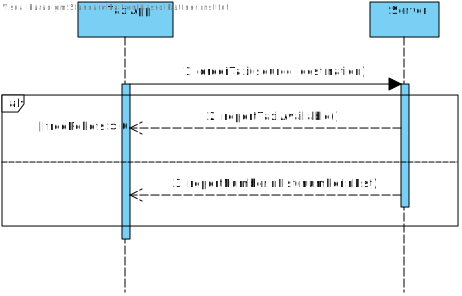
\includegraphics[width=0.9\textwidth]{img/2-Entwurf-RecieveOrder-Taxi}
	\caption{\emph{RecieveOrder-Taxi}-Sequenzdiagramm}
	\label{SequenzDiagrammInteraktion}
\end{figure}

\begin{figure}[H]
	\centering
	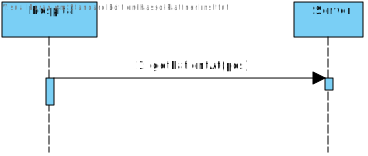
\includegraphics[width=0.9\textwidth]{img/2-Entwurf-RecieveOrder-Hosp}
	\caption{\emph{SEntwurf-RecieveOrder-Hosp}-Sequenzdiagramm}
	\label{SequenzDiagrammInteraktion}
\end{figure}



\subsection*{Interaktion bei Ausführung von \emph{Receive Boarding Confirmation \& Receive Arrival Notification}}

Alle Prozesse laufen wie ersichtlich über den Server, der wiederum die RobotUnit fernsteuert. 
So wird sowohl für Receive Boarding Confirmation( Use Case 1.3) erst vom Hospital oder der TaxiApp an den Server zurückgemeldet, dass sich der Patient oder der Costumer an Bord befindet, bevor die Fahrt aufgenommen werden kann. 
In gleichem Weise wird dem Server mit Receive Arrival Notification(UseCase 1.5) zurückgemeldet,das die RobotUnit wieder für weitere Einsätze verfügbar ist, sobald der Costumer die RobotUnit verlassen hat.  \\

\begin{figure}[H]
	\centering
	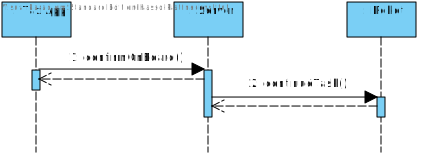
\includegraphics[width=0.9\textwidth]{img/2-Entwurf-ReceiveBoardingConfirmation-taxi}
	\caption{\emph{ReceiveBoardingConfirmation-taxi}-Sequenzdiagramm}
	\label{SequenzDiagrammInteraktion}
\end{figure}

\begin{figure}[H]
	\centering
	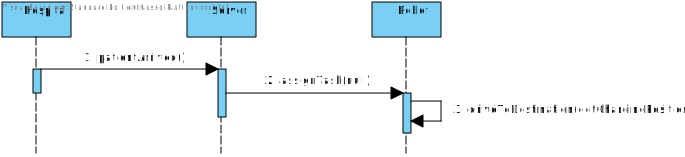
\includegraphics[width=0.9\textwidth]{img/2-Entwurf-ReceiveUnloadConfirmation-hospital}
	\caption{\emph{ReceiveUnloadConfirmation-hospital}-Sequenzdiagramm}
	\label{SequenzDiagrammInteraktion}
\end{figure}


\subsection*{Interaktion bei Ausführung von \emph{Use Cases Perfom Task \& Continue Task}}
Konkret wird die RobotUnit dabei über die UseCases Perfom Task(Use Case 2.2) und Continue Task( Use Case 2.3) eine Task(Parameter) zugewiesen, die solange ausgeführt, bis der der RobotUnit eine Abbruch Task zugewiesen wird oder das Ziel wiederum erfolgreich erreicht wurde und dies an den Server zurückgemeldet werden kann. \\

\begin{figure}[H]
	\centering
	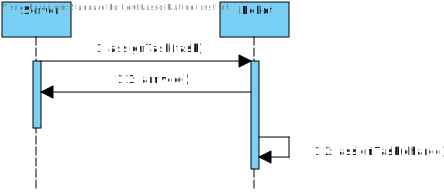
\includegraphics[width=0.9\textwidth]{img/2-Entwurf-PerformTask}
	\caption{\emph{Perform Task}-Sequenzdiagramm}
	\label{SequenzDiagrammInteraktion}
\end{figure}

\subsection* Die weiteren UseCases sind diesen untergeordnet; enthalten entweder nur einseitige Server/RobutUnit Kommunikation, wie zum Beispiel bei Request Repair( Use Case 1.6) oder haben ihren Fokus vor allem auf den Wechselwirkungen innerhalb der Robot Unit( Siehe dazu Kapitel 8). \\


\newpage
\section{Komponentenschnittstellen}

%3.1 Datentypen
\subsection{\textit{Datentypen}}
Die in Abbildung \ref{KomponentenschnittstellenDiagramm} dargestellten Datentypen werden von den Schnittstellen der eingeführten Komponenten verwendet. 

Die Aufgabe des Datentyps \emph{SensorData} ist primär, die Koordination mit dem Server zu unterstützen, um festzustellen, inwieweit eine Zielposition gut erreicht werden kann. Dazu besitzt er als Attribute die Orientierungsrichtung im Koordinatensystem, den Batteriestatus und zuletzt Attribute der Datentypen \emph{Position} und \emph{Destination}. \emph{Position} besitzt wiederum die Koordinaten x und y, die einen beliebigen Punkt im Bereich des Einsatzgebietes des Roboters darstellen. Um Redundanz zu vermeiden sind \emph{Destination} und \emph{Position} über keine zusätzliche Klassendiagrammbeziehung verknüpft. Zielpunkte erben von \emph{Position} und existieren zur Spezifikation, um welche Art Zielpunkt es sich handelt: Also zum Beispiel eine allgemeine \emph{Destination} oder den \emph{Charger}.
	
	\begin{figure}[H]
		\centering
		\includegraphics[width=0.75\textwidth]{img/3-Zusatzklassen}
		\caption{Datentypen, die in Komponentenschnittstellen verwendet werden}
		\label{KomponentenschnittstellenDiagramm}
	\end{figure}

%3.2 Interfaces
\subsection{\textit{Interfaces}}
	%3.2.1 ISensorData
	\subsubsection{\textit{Interfaces}}
	Dieses \textit{Interface} wird vom \textit{Robot} angeboten, um dem Server alle Sensordaten zu senden. Der Server kann anhand diesen jederzeit feststellen, in welchem Zustand sich der \textit{Robot} befindet um diesem dann eine \textit{Task} zuzuweisen.
	\begin{figure}[H]
	\centering
	\includegraphics[width=0.75\textwidth]{img/1-Entwurf-3-1_ISensorData}
	\caption{\textit{Interface} ISensorData}
	\label{ISensorData}
	\end{figure}
	
	%3.2.2 ITask
	\subsubsection{\textit{Interfaces}}
	Dieses \textit{Interface} wird vom \textit{Robot} angeboten, um Tasks zu erhalten. Der Server kann somit ohne Probleme \textit{Tasks} dem \textit{Robot} zuweisen. Hierbei findet eine Unidirektionale Kommunikation zwischen Server und Robot statt.
	\begin{figure}[H]
	\centering
	\includegraphics[width=0.75\textwidth]{img/1-Entwurf-3-1_ITask}
	\caption{\textit{Interface} ITask}
	\label{ITask}
	\end{figure}

\newpage
%4
\section{Konkrete Architektur}

Abbildung \ref{KomponentendiagrammKonkret} zeigt das konkrete, auf dem abstrakten Komponentendiagramm aus Kapitel 1 aufbauende, Komponentendiagramm.

\begin{figure}[H]
	\centering
	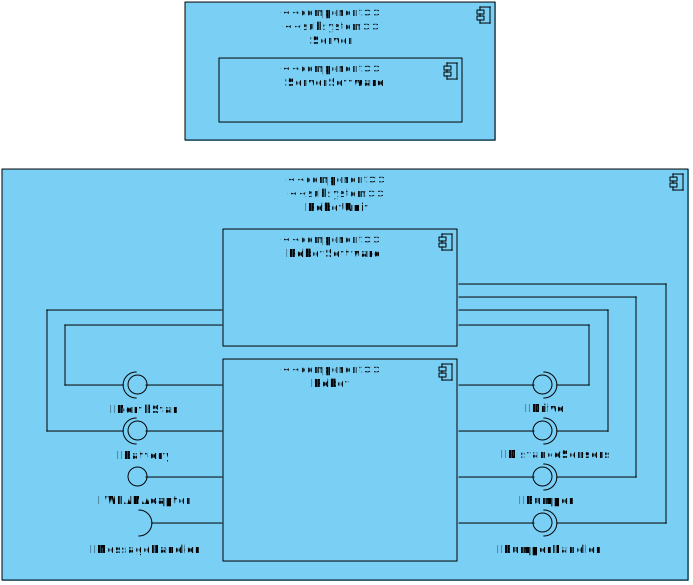
\includegraphics[width=1\textwidth]{img/4}
	\caption{Konkretes Komponentendiagramm}
	\label{KomponentendiagrammKonkret}
\end{figure}

%4.1 Server Software
\subsection{\textit{ServerSoftware}}
\begin{figure}[H]
\centering
\includegraphics[width=0.7\textwidth]{img/51}
\caption{Komponentendiagramm für den \emph{Server}}
\label{KomponentendiagrammKonkretServer}
\end{figure}
Abbildung \ref{KomponentendiagrammKonkretServer} zeigt das konkrete Komponentendiagramm für die Komponente \emph{Server}. Die \emph{ServerSoftware} tätigt in der aktuellen nullten Ausbaustufe direkt Aufrufe an den \textit{Robot}, 
um den besten \textit{Robot} für eine \textit{Destination} zu ermitteln und einem \textit{Robot} eine \textit{Destination} zuzuweisen.

%4.2 Robot Software
\subsection{\textit{RobotSoftware}}
\begin{figure}[H]
	\centering
	\includegraphics[width=1\textwidth]{img/52}
	\caption{Komponentendiagramm für den \emph{Robot}}
	\label{KomponentendiagrammKonkretRobot}
\end{figure}
In Abbildung \ref{KomponentendiagrammKonkretRobot} ist das konkrete Komponentendiagramm der \emph{Robot}-Komponente dargestellt. \emph{RobotSoftware} ist für die Steuerung der \textit{RobotUnit} zuständig. Die von der abstrakten Hardware 
des \textit{Robot} angebotenen, vorgegebenen Interfaces \textit{INorthStar, IBattery, IDrive, IDistanceSensors, IBumper} sowie 
\textit{IBumperHandler} werden dabei von der \textit{Robot}-Komponente für die konkrete Steuerung der \textit{RobotUnit} genutzt.

\newpage
\section{Komponenten}

%5.1 Server Software
\subsection{Komponente \textit{ServerSoftware}}
\begin{figure}[H]
\centering
\includegraphics[width=0.75\textwidth]{img/51.svg}
\caption{\textcolor{blue}{Server Software}}
\label{KomponentenStruktur1}
\end{figure}
Die Komponente \textit{ServerSoftware} umfasst 4 Klassen: \textit{TaskSystem}, \textit{Destination}, \textit{RobotControlSystem} und \textit{Virtual Robot}.
Das \textit{TaskSystem} verwaltet die \textit{Tasks}, in der nullten Ausbaustufe fallen dabei allerdings noch nicht viele Aufgaben an, 
da es keine Priorisierungen, unterschiedliche Arten von \textit{Tasks} oder dergleichen gibt. Die Klasse \textit{Destination} ist die Klasse 
der Aufgaben, die vom \textit{TaskSystem} verwaltet werden. Das \textit{RobotControlSystem} verteilt die \textit{Tasks} auf die \textit{Robots}. 
Dabei findet die Auswahl anhand der zurückgegebenen \textit{SensorData} der einzelnen \textit{Robots} statt. Bei \textit{VirtualRobot} handelt 
es sich um eine Kapselung der Kommunikation mit den \textit{Robots}. Hier werden alle von der Komponente \textit{Robot} bereitgestellten 
\textit{Interfaces} implementiert.
%5.1 Robot Software
\subsection{Komponente \textit{RobotSoftware}}
\begin{figure}[H]
\centering
\includegraphics[width=0.85\textwidth]{img/52.svg}
\caption{\textcolor{blue}{Durch eigene Diagramm ersetzen}}
\label{KomponentenStruktur2}
\end{figure}
Die Komponente \textit{RobotSoftware} enthält 3 Klassen: \textit{DrivingSystem}, \textit{RobotController} und \textit{Destination}. 
Das \textit{DrivingSystem} stellt eine Abstraktion der Hardware dar und wird dazu genutzt, Ziele anzufahren und Dabei, 
falls nötig, Hindernisse zu umfahren. Dazu greift es auf die von der Hardware bereitgestellten \textit{Interfaces} zurück. 
Um auf Kollisionen reagieren zu können, implementiert das \textit{DrivingSystem} die Schnittstelle \textit{IBumperHandler}
Der \textit{RobotController} stellt die Interfaces \textit{ITask} und \textit{ISensordata} (dem Server) zur Verfügung und verwaltet den gerade 
zu absolvierenden \textit{Task}. Zur Messwertübermittlung greift er zum einen auf das \textit{DrivingSystem} und zum anderen auf das 
von der Hardware angebotenen \textit{Interface} \textit{IBattery} zu.


\newpage
\section{Paketstruktur}
\textcolor{blue}{\textit{Dieser Abschnitt beschreibt im Wesentlichen eine grobe Zerlegung der zu entwickelnden Anwendung in Pakete und deren Zusammenhänge. Dabei sollen Zusammenhänge und Abhängigkeiten zwischen den Paketen beschrieben werden.\\\\
Die hier definierten Pakete sind logische Einheiten oder gemeinsam genutzte Einheiten, die aus beliebig vielen Klassen bestehen können, welche gemeinsam die Funktionalität durch das Paket zusammenfassen. Die Aufteilung von Klassen zu Paketen muss sich dabei nicht an den strukturellen Eigenschaften der Architektur (z.B. Komponenten) orientieren. Vielmehr soll die Zerlegung in Pakete der besseren Strukturierung, Organisation, Arbeitsteilung bei Implementierung und Übersichtlichkeit der in der gesamten Architektur verwendeten Klassen dienen.\\\\
Das folgende Paketdiagramm führt Pakete ein und beschreibt ihre Abhängigkeiten. 
}}
%TODO: Text

\begin{figure}[H]
\centering
\includegraphics[width=0.8\textwidth]{../images/Iteration0_Entwurf_6_Paketdiagramm}
\caption{Abbildung 6.1: Paketdiagramm}
\label{Paketstruktur}
\end{figure}

\newpage
\section{Paketdetails}
\begin{figure}[H]
\centering
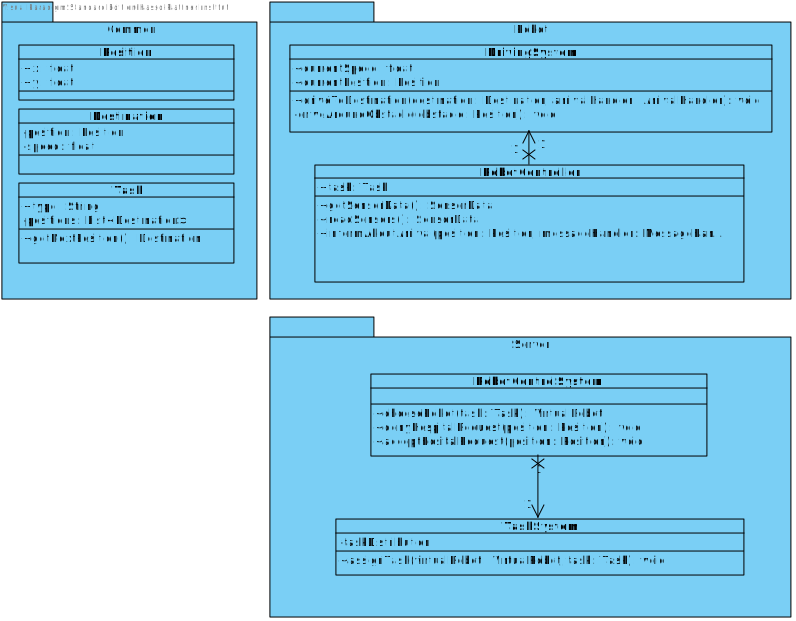
\includegraphics[height=0.75\linewidth, angle=90]{img/7-paketdetails}
\caption{Klassendiagramm zur detaillierten Beschreibung der strukturellen Gliederung}
\label{Paketdetails}
\end{figure}
%\pagebreak

%7.1 Paket Robot
\subsection{Paket \textit{RobotUnit}}
	Im Folgenden beschreiben wir die elementaren Klassen des Pakets \textit{RobotSoftware} 
	und ihre zugehörigen wichtigsten Methoden, sowie ihre Interaktion untereinander. 


	%7.1.1 RobotController
	\subsubsection{Beschreibung der Klasse \textit{RobotController}}
%		\begin{figure}[H]
%		\centering
%		\includegraphics[width=0.6\textwidth]{../images/Iteration0_Entwurf_7-1-1_Klasse_RobotController}
%		\caption{\textcolor{blue}{Durch eigene Diagramme ersetzen}}
%		\label{BeschreibungKlasse1}
%		\end{figure}
		
		%#destination : Destination
		Die Klasse \textit{RobotController} ist die Hauptklasse der \textit{RobotSoftware}, 
		da sie den aktuellen Zustand der \textit{RobotUnit} kapselt.
		Sie verwaltet alle internen Vorgänge der \emph{RobotUnit} und speichert den gerade verfolgten \textit{Task}. Dabei gibt es drei mögliche Zustände: 1. Die \emph{RobotUnit} verfolgt eine vom \emph{Server} auferlegte \emph{Task}. 2. Die \emph{RobotUnit} hat sich selbstständig den \emph{Task} gegeben, einen \emph{Charger} aufzusuchen. 3. Es gibt derzeit keinen \emph{Task}.

			%7.1.1.1 #collectSensorData():void
			\paragraph{Beschreibung der Methode \texttt{readSensors}}
			Der Server kann einen \textit{Robot} dazu auffordern, ihm seine Sensordaten zu schicken. 
			Der \textit{Robot} fragt dann seine Hardwareschnittstelle mittels der Methode \texttt{readSensors} 
			nach seiner Position und seinem Akkustand an und gibt diese Informationen zurück an den \textit{Server}. 
			Dazu wird natürlich zunächst eine \textit{Message} verfasst, welche dann über den \textit{IWlanAdapter} verschickt wird.
			
			\paragraph{Beschreibung der Methode \texttt{setTask}}
			Diese Methode wird aufgerufen, wenn der \textit{Robot} einen neuen Task erhält. Wenn der \textit{Robot} davor keinen \textit{Task} hatte, wird dieser einfach ausgeführt. Wenn der übergebene \textit{Task} \texttt{null} ist, nimmt der \textit{Robot} fahrt zur Ladestation auf. Wenn der \textit{Robot} gerade einen \textit{TaxiCustomer} an bord hat und in dieser Methode einen Krankenhaustransport als \textit{Task} erhält, wird der \textit{TaxiCustomer} abgeladen, und der Krankenhaustransport wird ausgeführt.
			
	\subsubsection{Beschreibung der Klasse \textit{VirtualServer}}
	Die Klasse \textit{VirtualServer} ist die Klasse, welche die Remote-Procedure-Calls von der Seite des \textit{Robots} implementiert. \textit{VirtualServer} implementiert unsere in 3. definierten Interfaces \textit{IRepair} und \textit{IArrivalNotification}. Alle Methoden in dieser Klasse verfassen natürlich eine \textit{Message} und nutzen dann die \textit{IWlanAdapter}-Schnittstelle, um diese an den \textit{Server} zu schicken.
	
			\paragraph{Beschreibung der Methode \texttt{informAboutArrival}}
			Diese Methode wird immer dann aufgerufen, wenn der \textit{Robot} die nächste \textit{Position} von seinem aktuellen \textit{Task} erreicht hat.  Da der \textit{Server} weiß, welcher \textit{Task} von welchem \textit{Robot} ausgeführt wird, muss \texttt{informAboutArrival} keine Parameter übergeben.
	
			\paragraph{Beschreibung der Methode \texttt{requestRepair}}
			Diese Methode wird dann von einen \textit{Robot} aufgerufen, wenn er nach einem Unfall kaputt ist. Der \textit{Robot} verfasst dafür eine \textit{Message} an den \textit{Server}, woraufhin auf dem \textit{Server} der \textit{Task}, den der kaputte \textit{Robot} gerade ausführen sollte, neu verteilt. In seiner Prioritätsstufe ist dieser \textit{Task} dann an erster Stelle, und wird nicht wieder hinten angestellt. Zusätzlich wird auf dem \textit{Server} dann die Methode \texttt{notifyRepairService} aufgerufen.		
			
	%7.1.2 DrivingSystem
	\subsubsection{Beschreibung der Klasse \textit{DrivingSystem}}
%		\begin{figure}[H]
%		\centering
%		\includegraphics[width=0.6\textwidth]{../images/Iteration0_Entwurf_7-1-2_Klasse_DrivingSystem}
%		\caption{\textcolor{blue}{Durch eigene Diagramme ersetzen}}
%		\label{BeschreibungKlasse1}
%		\end{figure}
		
		%#currentSpeed:float
		Diese Klasse beschreibt den aktuellen Zustand des Fahrsystems des \textit{Robots}. 
		Es sind Informationen über die aktuelle Geschwindigkeit enthalten und die Methode, 
		die gerade ausgeführt wird, gibt Auskunft über die aktuelle Beschäftigung des \textit{Robots}.

			%7.1.2.1 	#driveToDestination(destination: Destination, arrivalHandler: ArrivalHandler): void
			\paragraph{Beschreibung der Methode \texttt{driveToDestination}}
			\begin{figure}[H]
			\centering
			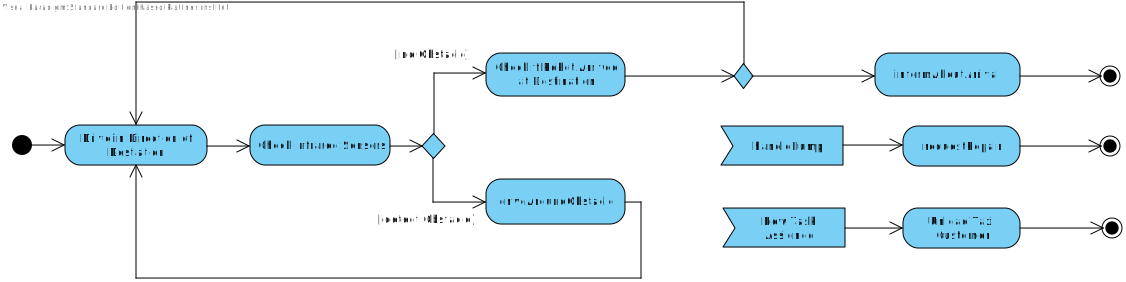
\includegraphics[width=1\textwidth]{img/7-1-methode_driveToDestination}
			\caption{Aktivitätsdiagramm zur Methode \texttt{driveToDestination}}
			\label{AktivitaetDriveToDestination}
			\end{figure}

			Wenn diese Methode aufgerufen wird, macht der \textit{Robot} sich auf den Weg zur 
			übergebenen \textit{Destination}. Wenn der \textit{Robot} an dieser \textit{Destination} 
			angekommen ist, wird die \texttt{arrive}-Methode des übergebenen \textit{ArrivalHandlers} ausgeführt. Wenn es sich bei der \textit{Destination} nicht um einen \textit{Charger} handelte, wird darin insbesondere über die von uns definierte Schnittstelle \textit{IArrivalNotifivation} der \textit{Server} über die Ankunft benachrichtigt. 
			Wenn sich ein \textit{Obstacle} auf dem Weg befindet, wird die Methode \texttt{driveAroundObstacle} 
			aufgerufen, bis das \textit{Obstacle} umfahren wurde.
			
			Abbildung \ref{AktivitaetDriveToDestination} zeigt ein entsprechendes Aktivitätsdiagramm.

			%7.1.2.2    -driveAroundObstacle(destination: Destination): void
			\paragraph{Beschreibung der Methode \texttt{driveAroundObstacle}}
			\begin{figure}[H]
			\centering
			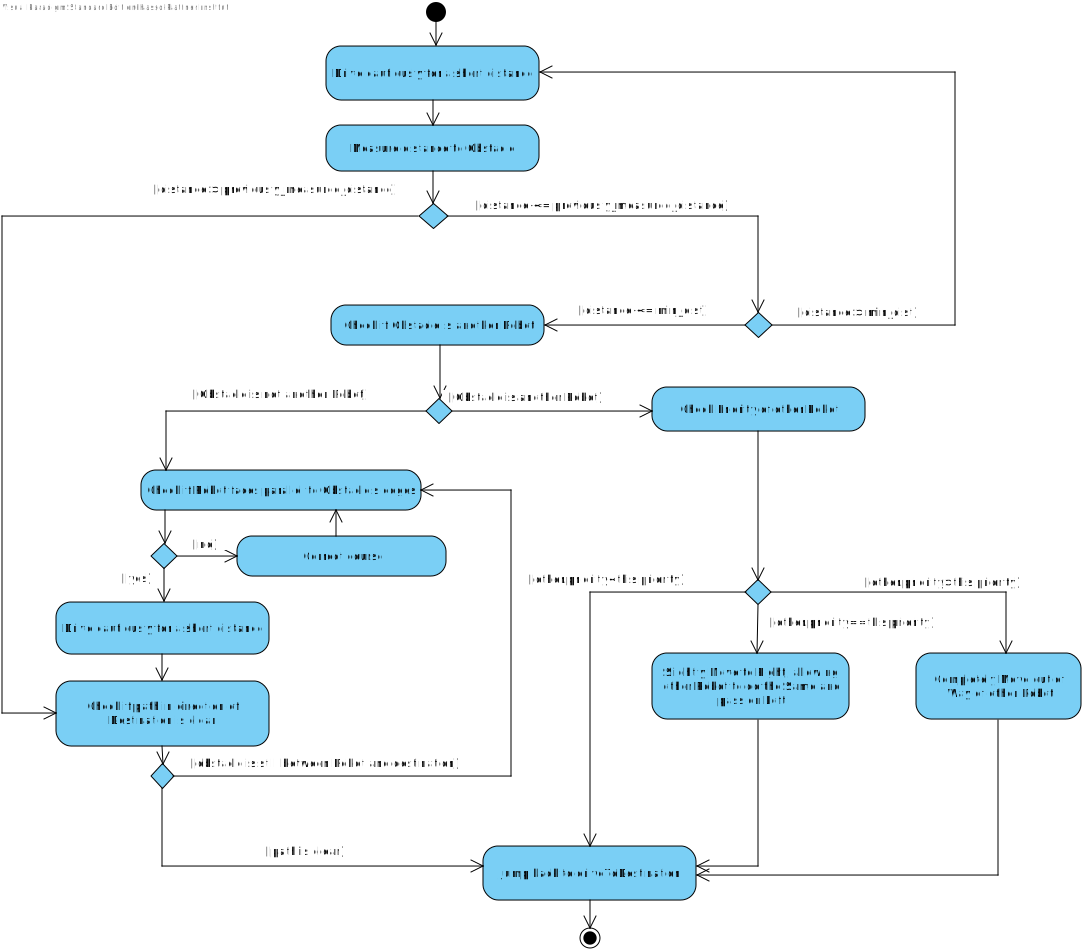
\includegraphics[width=0.95\textwidth]{img/1-Entwurf-7-driveAroundObstacle}
			\caption{Sequenzdiagramm zur Beschreibung der Methode \texttt{driveAroundObstacle}}
			\label{SequenzDriveAroundObstacle}
			\end{figure}

			Diese Methode wird von \texttt{driveToDestination} mit der Position eines \textit{Obstacles} aufgerufen, 
			wenn ein \textit{Obstacle} zu umfahren ist. 
			Im Spezialfall, dass es sich bei dem \textit{Obstacle} um einen anderen \textit{Robot} handelt, merken dies beide, wenn sie sich nähern und weichen beide nach rechts aus. 
			Im Allgemeinen entscheidet sich der \emph{Robot} zunächst, ob er links oder rechts an dem \textit{Obstacle} vorbeifährt, 
			und hält sich dann mithilfe seiner Sensoren immer auf einem bestimmten Abstand zum Hindernis, bis zwischen 
			\textit{Obstacle} und der Luftlinie zur \textit{Destination} genug Platz für den \textit{Robot} ist.
			
			Abbildung \ref{SequenzDriveAroundObstacle} zeigt ein entsprechendes Sequenzdiagramm. 
			Dabei ist \texttt{min\_dist} eine vorher festgelegte Konstante, welche die Mindestdistanz, die der \textit{Robot} halten muss, wenn er an einem \textit{Obstacle} vorbeifährt, speichert.
	
\pagebreak
	
%7.2 Paket Server
\subsection{Paket \textit{Server}}
%\begin{figure}[H]
%	\centering
%	\includegraphics[width=0.6\textwidth]{../images/Paketdetails.png}
%	\caption{\textcolor{blue}{HIER KOMMT DAS Server - PAKETDIAGRMAM HIN}}
%	\label{Paketdetails}
%	\end{figure}
	Im Folgenden werden die wichtigen Klassen des Pakets \textit{Server} 
	und ihre zugehörigen Methoden sowie ihre Interaktion untereinander beschrieben. 


	%7.2.1 TaskSystem
	\subsubsection{Beschreibung der Klasse \textit{TaskQueue}}
	
	Diese Klasse ist für die Verwaltung von \textit{Tasks} auf dem \textit{Server} zuständig. Prinzipiell ist hier eine Queue implementiert, welche aber noch über zusätzliche Funktionen, wie z.B \texttt{addTop} und \texttt{remove} verfügt. Ziel dieser Datenstruktur ist es, die Wartezeiten für mögliche Taxikunden fair zu handhaben und die Verteilung an die \textit{Robots} vorzunehmen.
	
			\paragraph{Beschreibung der Methode \texttt{add}}		
			\begin{figure}[H]
			\centering
			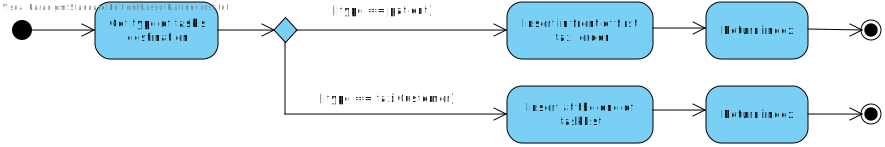
\includegraphics[width=0.95\textwidth]{img/add}
			\caption{Sequenzdiagramm zur Beschreibung der Methode \texttt{add}}
			\label{SequenzQueueAdd}
			\end{figure}
			
			Die Methode \texttt{add} dient dazu neue Tasks in die Warteliste einzufügen.
			
			\paragraph{Beschreibung der Methode \texttt{addTop}}		
%			\begin{figure}[H]
%			\centering
%			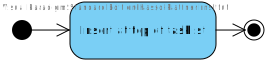
\includegraphics[width=0.95\textwidth]{img/addTop}
%			\caption{Sequenzdiagramm zur Beschreibung der Methode \texttt{addTop}}
%			\label{SequenzQueueAddTop}
%			\end{figure}			
			
			Mit der Methode \texttt{addTop} können \textit{Tasks} in die Queue hinzugefügt werden, die davor schon aktiv von einem \textit{Robot} bearbeitet wurden, dann aber durch einen Defekt dessen neu verteilt werden müssen. 
			Die Besonderheit dieser \textit{Tasks} ist, dass sie an den Anfang der Queue hinzugefügt werden müssen.
				
			\paragraph{Beschreibung der Methode \texttt{poll}}		
			\begin{figure}[H]
			\centering
			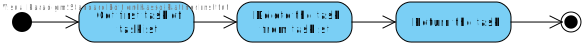
\includegraphics[width=0.95\textwidth]{img/2-Entwurf-poll}
			\caption{Sequenzdiagramm zur Beschreibung der Methode \texttt{poll}}
			\label{SequenzQueuePoll}
			\end{figure}			
			
			Die Methode \texttt{poll} gibt den nächsten zu bearbeitenden Task zurück und entfernt diesen aus der Queue.
				
			\paragraph{Beschreibung der Methode \texttt{remove}}		
			\begin{figure}[H]
			\centering
			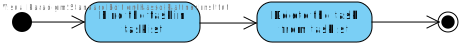
\includegraphics[width=0.95\textwidth]{img/2-Entwurf-remove}
			\caption{Sequenzdiagramm zur Beschreibung der Methode \texttt{remove}}
			\label{SequenzQueueRemove}
			\end{figure}			
			
			Die Methode \texttt{remove} entfernt einen spezifischen Task aus der Queue.
			
	%7.2.2 RobotControlSystem
	\subsubsection{Beschreibung der Klasse \textit{VirtualRobotManager}}
			\paragraph{Beschreibung der Methode \texttt{handleArrival}}
			\begin{figure}[H]
			\centering
			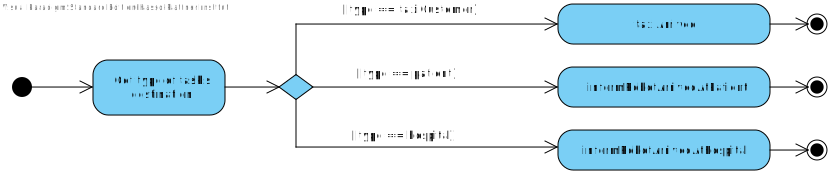
\includegraphics[width=0.95\textwidth]{img/HandleArrival}
			\caption{Sequenzdiagramm zur Beschreibung der Methode \texttt{handleArrival}}
			\label{SequenzQueuePoll}
			\end{figure}	
			Diese Methode wird immer dann aufgerufen, wenn der \textit{Server} eine \textit{Message} von einem \textit{Robot} erhält, welche von ihm über das von uns definierte Interface \textit{IArrivalNotification} gesandt wurde. Da der \textit{Server} eingespeichert hat, welchen \textit{Task} der \textit{Robot} gerade ausführt, müssen keine Parameter übergeben werden, sondern der \textit{Server} kann einfach nachschauen, welcher Typ von \textit{Destination} gerade erreicht wurde. Je nach Typ wird dann eine Benachrichtigung an die zugehörigen \textit{Customers} gesendet. Bei einem Taxiauftrag wird keine Nachricht an den Taxikunden geschickt, wenn dieser sein Ziel erreicht. Laut Aufgabenstellung ist eine Taxifahrt mit erreichen der \textit{Destination} des Taxikunden sofort beendet, ohne dass weitere Benachrichtigungen an den Taxikunden geschickt werden müssen.
			
			
			%7.2.1.1	~chooseRobot(destination: Destination): void
			\paragraph{Beschreibung der Methode \texttt{chooseRobot}}
			Die Methode \texttt{chooseRobot} wählt für den aktuell eingegangenen \emph{Task} einen \emph{Robot} aus. 
			Dazu fragt es die Sensorwerte der verschiedenen \emph{Robots} ab und wählt den am besten geeigneten aus.
				
			\begin{figure}[H]
			\centering
			\includegraphics[width=0.95\textwidth]{img/1-Analyse-3-Choose_Robot}
			\caption{Aktivitätsdiagramm zur Beschreibung der Methode \texttt{chooseRobot}}
			\label{SequenzQueueRemove}
			\end{figure}			
				
			\begin{figure}[H]
			\centering
			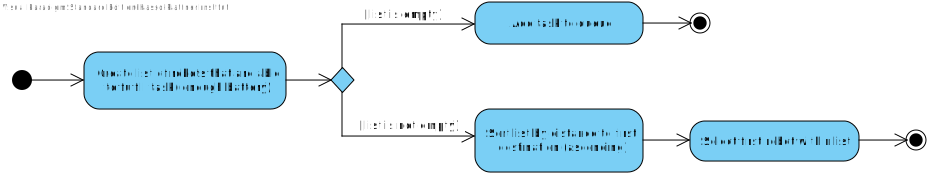
\includegraphics[width=0.95\textwidth]{img/2-Entwurf-SelectBestMatch}
			\caption{Aktivitätsdiagramm zur Beschreibung der Aktivität \texttt{selectBestMatch}}
			\label{SequenzQueueRemove}
			\end{figure}

			\paragraph{Beschreibung der Methode \texttt{notifyRepairService}}
			Wenn ein \textit{Robot} nach einem Zusammenstoß defekt ist, teilt er dies dem \textit{Server} unter Verwendung seiner Methode \texttt{requestRepair} mit.	Daraufhin erstellt der \textit{Server} einen neuen  \textit{Task}, der am Unfallort des \textit{Robots} beginnt. Der \textit{Customer}, der an Bord des verunglückten \textit{Robots} war, wird also nicht im Stich gelassen. Der neue \textit{Task} wird mit der Methode \texttt{addTopOfType} in die \textit{TaskPriorityQueue} eingefügt, um die Wartezeit dieses \textit{Customers} zu minimieren. Daraufhin benachrichtigt der \textit{Server} einen System-externen Servicedienst, und übergibt diesem die Position des Unfallorts. Nach unserer Annahme aus der Analyse wird der dort verunglückte \textit{Robot} dann nach einer endlichen Zeit wieder vom System benutzbar sein.
			
			
			
	\subsubsection{Beschreibung der Klasse \textit{VirtualRobotUnit}}
	Die Klasse \textit{VirtualRobotUnit} ist die Umsetzung der Remote-Procedure-Calls von der Seite des \textit{Servers}. Diese Klasse implementiert die Methoden der von uns in 3. beschriebenen Interfaces \textit{ITask} und \textit{ISensorData}. Da diese Klasse auch die Repräsentation des \textit{Robots} auf dem \textit{Server} ist, werden hier auch Zustand des zugehörigen \textit{Robots}, insbesondere aktuell auszuführenden \textit{Task}, gespeichert. Alle Methoden dieser Klasse werden im \textit{Server} aufgerufen und Verfassen zunächst eine \textit{Message}, welche dann über die \textit{IWlanAdapter}-Schnittstelle verschickt werden und daraufhin die zugehörigen Lokalen Methoden auf den \textit{Robots} aufgerufen werden.
	
			\paragraph{Beschreibung der Methode \texttt{assignTask}}
			Mit dieser Methode teilt der \textit{Server} einem \textit{VirtualRobot} einen neuen \textit{Task} zu, der dann von dem zugehörigen \textit{Robot} ausgeführt wird. Auf dem zugehörigen \textit{Robot} wird dafür die Methode \texttt{setTask} aufgerufen.
			
			\paragraph{Beschreibung der Methode \texttt{continueTask}}
			Diese Methode wird zum Beispiel dann aufgerufen, wenn der \textit{Server} die Nachricht erhalten hat, dass sich der \textit{Customer} nun an Bord des \textit{Robots} befindet. Daraufhin wird eine \textit{Message} an den zu diesem \textit{VirtualRobot} zugehörigen \textit{Robot} geschickt, der ihn wissen lässt, dass er die nächste \textit{Destination} in seinem aktuellen \textit{Task}			
			
			\paragraph{Beschreibung der Methode \texttt{getSensorData}}
			Der \textit{Server} möchte im Rahmen von \texttt{Choose Robot} Informationen über den Akkustand und die Position von allen \textit{Robots} erhalten. Dazu wird auf jedem \textit{VirtualRobot} diese Methode aufgerufen, bei der über die \textit{IWlanAdapter}-Schnittstelle eine entsprechende \textit{Message} an den jeweils zugehörigen \textit{Robot} geschickt wird. Diese \textit{Robots} rufen dann die Methode \texttt{readSensors} auf.

\newpage
\section{Abläufe}

Während in Kapitel 2 die Interaktion der Hauptkomponenten \emph{Server} und der \emph{RobotUnit} abgehandelt wurden, werden im Folgenden die Abläufe der Use Cases genauer spezifiziert und auch interne Komponentenabläufe beschrieben, im Speziellen die Abläufe innerhalb der \emph{RobotUnit}.
	
	\subsection*{Interaktion bei Ausführung von Use Case 1 – \emph{Choose Path around Obstacle} und Use Case 2 – \emph{Drive around Obstacle}}
	Sowohl der Use Case \emph{Choose Path around Obstacle} als auch der Use Case \emph{Drive around Obstacle} sind beide Teil des Geschäftsprozesses \emph{Drive to Destination}. Abbildung \ref{UmfahrenvonstatichenObjekten} zeigt ein Sequenzdiagramm des Use Case \emph{Drive around Obstacle}. Wie schon der Name beschreibt, befindet sich die \emph{RobotUnit} dabei in einem Fahrvorgang, der vorher konkret mit der Zielposition und der Geschwindigkeit vom \emph{Server} eingestellt wurde. 
	
	So reagiert intern seine Software mit dem \emph{IDistanceSensor}, wenn ein Hindernis um ihn herum auftaucht und dieses mit Hilfe der durch die Sensoren gesammelten Informationen umfahren werden muss. Dabei muss der \emph{Robot} ausdrücklich zwischen einem \emph{Robot} und einem unbeweglichen Hindernis unterscheiden, um so vorherzubestimmen, wie eine optimale Ausweichbewegung aussieht. Auch wenn der \emph{IDistanceSensor} die vollständige Umgebung um den \emph{Robot} wahrnehmen kann, bezieht sich dies jedoch primär auf vor dem \emph{Robot} liegende Hindernisse. Dieser Prozess ist Bestandteil des Use Case \emph{Choose Path around Obstacle} und geht dann in den Use Case \emph{Drive Around Obstacle} über. 
	
	Der \emph{Robot} koordiniert sich dort mit seiner \emph{IDrive}-Komponente und seinen Sensoren, um langsam an einem unbeweglichen Objekt vorbeizufahren. Dabei fährt er immer eine kleine Distanz parallel zur Kante des \emph{Obstacles} und prüft, ob der Weg zum Ziel wieder frei ist. Ist dies der Fall, nimmt er den Fahrtprozess wieder auf. Erkennen sich zwei \emph{Robots} hingegen gegenseitig als Hindernis, weichen beide mit Hilfe ihrer \emph{IDrive}-Komponente jeweils nach rechts aus und nehmen anschließend den normalen Fahrbetrieb wieder auf. \\
	
	\subsection*{Interaktion bei Ausführung von Use Case 3 – \emph{Read Sensors}}
In Abbildung \ref{ReadSensors} wird der reine Anfrageprozess zwischen \emph{Server} und der \emph{RobotUnit} aus Kapitel 2 erweitert. Nach der Anfrage wird der \emph{Robot} alle nötigen Informationen nacheinander abfragen: Sowohl die \emph{Position} als auch die Orientierungsrichtung werden von der \emph{INorthStar}-Komponente zurückgeliefert. Für den Batteriestatus muss die \emph{IBattery}-Komponente angefragt werden. Erst wenn alle Informationen als Gesamtpaket bereitstehen, können sie an den Server zurückgemeldet werden.
\\
	\begin{figure}[H]
		\centering
		\includegraphics[width=0.95\textwidth]{img/1-Entwurf-8-DriveArroundObstacle}
		\caption{Sequenzdiagramm von \emph{Drive arround Obstacle}}
		\label{UmfahrenvonstatichenObjekten}
	\end{figure}
	\vspace{1cm}
	
	\begin{figure}[H]
		\centering
		\includegraphics[width=1\textwidth]{img/0-Entwurf-8-ReadSens}
		\caption{Sequenzdiagramm von \emph{Read Sensors}}
		\label{ReadSensors}
	\end{figure}
	
	
	
	\subsection*{Interaktion bei Ausführung von Use Case 4 – \emph{Charging}}
	Beim Use Case \emph{Charging} (Sequenzdiagramm in Abbildung \ref{Charging}) findet keine Kommunikation mit der Komponente \emph{Server} statt, dafür allerdings zwischen der \emph{RobotUnit} und der \emph{Charging\-Station}. Hat der \emph{Robot} einen bestimmten kritischen Ladestand erreicht (den er regelmäßig überprüft), läuft er die \emph{Charging\-Station}-Komponente an. Der Ladevorgang triggert automatisch, sobald der \emph{Robot} die \emph{Position} der Ladestation erreicht hat, und interagiert solange mit ihr bis seine Batterie wieder aufgeladen ist. Innerhalb des \emph{Robots} werden zum Anfahren der \emph{ChargingStation} die Komponenten \emph{IBattery} mit der \emph{Position} der robotereigenen Ladestation und \emph{IDrive} benötigt. Konkret: Wenn \emph{IDrive} \texttt{arrived()} zurückgibt, kann der Ladevorgang begonnen werden.
	\vspace{1cm}
	
	\begin{figure}[H]
		\centering
		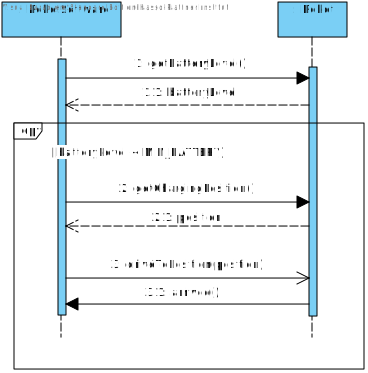
\includegraphics[width=0.65\textwidth]{img/0-Entwurf-8-Charging}
		\caption{Sequenzdiagramm von \textit{Charging}}
		\label{Charging}
	\end{figure}

\newpage
\section{Produkteinsatz}
\textcolor{blue}{\textit{In diesem Abschnitt wird der geplante Einsatz des zu entwickelnden Produktes beschrieben. Dies umfasst insbesondere die Systemumgebung in der das Produkt eingesetzt werden soll und die Zuordnung der Software zu dieser.
}}

\begin{figure}[H]
\centering
\includegraphics[width=0.75\textwidth]{img/Produkteinsatz.png}
\caption{\textcolor{blue}{Durch eigene Diagramme ersetzen}}
\label{Produkteinsatz}
\end{figure}


\end{document}
